\documentclass[12pt,titlepage]{beamer}
\usepackage{pdfpcnotes}
% language stuff
\usepackage{german}           % deutsche Überschriften etc.
\usepackage[utf8]{inputenc} % direkte Einbgabe von Umlauten

% Layout-Einstellungen
\usepackage{parskip}          % Abstand statt Einrückung
\frenchspacing                % no extra space after periods
\usepackage{parskip}          % paragraph gaps instead of indentation
\usepackage{times}            % default font Times
\tolerance=9000               % avoid words across right border
% miscellaneous<
\usepackage{hhline}           % double lines in tables
\usepackage{amsfonts}         % real numbers etc.
\usepackage[rightcaption]{sidecap} % figure captions on the right (optional)
\usepackage{hyperref}         % for URLs
\usepackage{listings}         % for code samples
 \lstset{breaklines=true,tabsize=1}
\usepackage{etoolbox}
\usepackage{multirow}
\usepackage{tabularx}
\usepackage{amsmath}
\usepackage{multirow}
\usepackage{pbox}
\usepackage{graphicx}
\usepackage[vlined]{algorithm2e}
\usepackage{svg}
\usepackage{tikz}

\definecolor{HIGHLIGHTCOLOR}{rgb}{0.13333333333333333,0.8156862745098039,0.09019607843137255}



\defbeamertemplate{section page}{mine}[1][]{%
  \begin{centering}
    {\usebeamerfont{section name}\usebeamercolor[fg]{section name}#1}
    \vskip1em\par
    \begin{beamercolorbox}[sep=12pt,center]{part title}
      \usebeamerfont{section title}\insertsection\par
    \end{beamercolorbox}
  \end{centering}
}

\AtBeginSection{\setbeamertemplate{section page}[mine]\frame{\sectionpage}}


\makeatletter
\patchcmd{\insertverticalnavigation}%
{\ifx\beamer@nav@css\beamer@hidetext{\usebeamertemplate{section in sidebar}}\else{\usebeamertemplate{section in sidebar shaded}}\fi}%
{{\usebeamertemplate{section in sidebar}}}{}{}
\makeatother



% Hier bei Bedarf die Seitenränder einstellen
%\geometry{a4paper}
\usetheme{Hannover}
\usecolortheme{rose}
\begin{document}
	\title{Netzoptimierung und Lernalgorithmen für Neuronale Netze}
	\author{Michael Känmmerer}
	\date{\today}
	\institute{}
%------------------------------------------------Folie1----------------------------------------------------------
	\begin{frame}
		\maketitle
	\end{frame}
	\section{Grundlagen}
	\subsection{Allgemeiner Aufbau neuronaler Netze}
		
	\begin{frame}
	\frametitle{Allgemeiner Aufbau neuronaler Netze}
	Künstliche neuronale Netze versuchen Lernmodelle des Gehirns nachzubilden.
	
	Es existieren verschiedenste Lernverfahren zum trainieren von neuronalen Netzen.
	
	Neuronale Netze können vielseitig eingesetzt werden, zum Beispiel in der Mustererkennung.
	
	\end{frame}
	\begin{frame}
	\frametitle{Allgemeiner Aufbau neuronaler Netze}
Zur Abbildung der funktionsweise existiert ein mathematisches Modell:
\begin{figure}[H]
	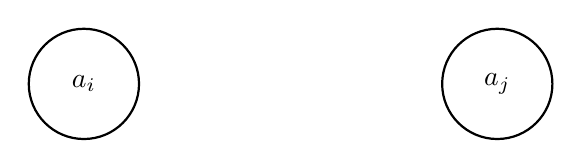
\begin{tikzpicture}[scale=0.7]
	
	\draw[thick](3.5,0)circle(1) node{$a_i$};
	
	\draw[thick](11,0)circle(1) node{$a_j$};
	
	\end{tikzpicture}
\end{figure}
1. Jedes Neuron hat einen Aktivierungszustand $a_i(t)$ zum Zeitpunkt t.
\end{frame}
\begin{frame}
\frametitle{Allgemeiner Aufbau neuronaler Netze}
\begin{figure}[H]
	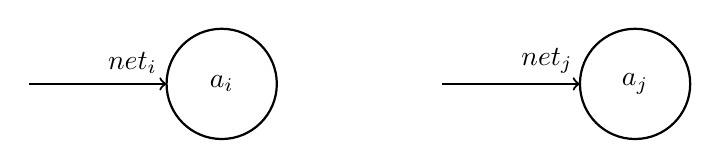
\begin{tikzpicture}[scale=0.7]
	\draw[->,thick](0,0)--(2.5,0)node[above right, midway]{$net_i$};
	\draw[thick](3.5,0)circle(1) node{$a_i$};
	\draw[->,thick](7.5,0)--(10,0)node[above right, midway]{$net_j$};
	\draw[thick](11,0)circle(1) node{$a_j$};
	\end{tikzpicture}
\end{figure}
2. Jedes Neuron hat eine Aktivierungsfunktion $f_{act}$ zur Berechnung eines neuen Aktivierungszustandes aus er Eingabe $net_i$ und eines Schwellwerts.
\end{frame}
\begin{frame}
\frametitle{Allgemeiner Aufbau neuronaler Netze}
\begin{figure}[H]
	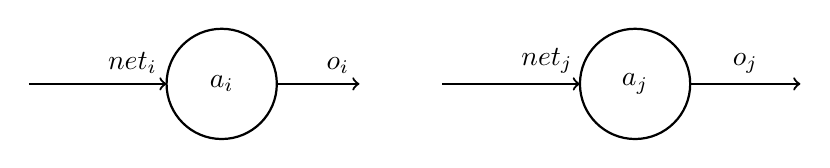
\begin{tikzpicture}	[scale=0.7]
	\draw[->,thick](0,0)--(2.5,0)node[above right, midway]{$net_i$};
	\draw[thick](3.5,0)circle(1) node{$a_i$};
	\draw[->,thick](4.5,0)--(6,0)node[above left]{$o_i$};
	\draw[->,thick](7.5,0)--(10,0)node[above right, midway]{$net_j$};
	\draw[thick](11,0)circle(1) node{$a_j$};
	\draw[thick,->](12,0)--(14,0) node[above,midway]{$o_j$};
	\end{tikzpicture}
\end{figure}
3. Jedes Neuron hat eine Ausgabefunktion $f_{out}$ die aus dem Aktivierungszustand die Ausgabe $o$ des Neurons berechnet.
\end{frame}
\begin{frame}
\frametitle{Allgemeiner Aufbau neuronaler Netze}
\begin{figure}[H]
	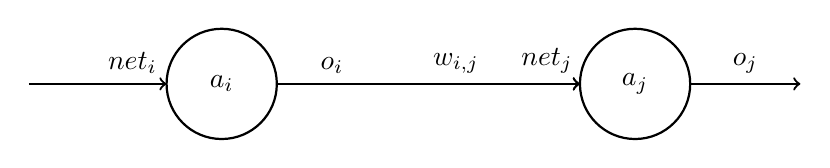
\begin{tikzpicture}[scale=0.7]
	\draw[->,thick](0,0)--(2.5,0)node[above right, midway]{$net_i$};
	\draw[thick](3.5,0)circle(1) node{$a_i$};
	\draw[thick](4.5,0)--(5.5,0)node[above]{$o_i$};
	\draw[->,thick](5.5,0)--(10,0)node[midway, above]{$w_{i,j}$};
	\draw[->,thick](7.5,0)--(10,0)node[above right, midway]{$net_j$};
	\draw[thick](11,0)circle(1) node{$a_j$};
	\draw[thick,->](12,0)--(14,0) node[above,midway]{$o_j$};
	\end{tikzpicture}
\end{figure}
4. Die Neuronen sind über ein Netzwerk aus Synapsen $w_{ij}$ miteinander verbunden.
\end{frame}
\begin{frame}
\frametitle{Allgemeiner Aufbau neuronaler Netze}
	\begin{figure}[H]
	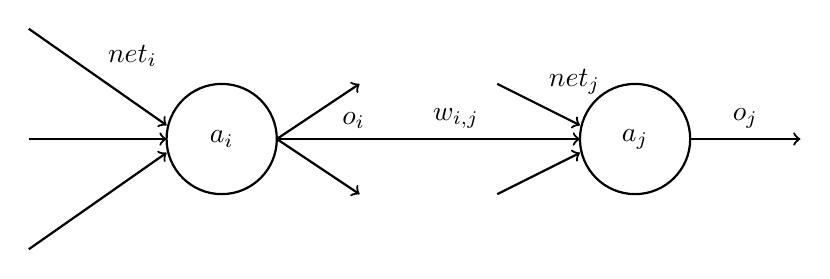
\begin{tikzpicture}	[scale=0.7]
	\draw[->,thick](0,0)--(2.5,0);
	\draw[->,thick](0,2)--(2.5,0.25)node[above right, midway]{$net_i$};
	\draw[->, thick](0,-2)--(2.5,-0.25);
	\draw[thick](3.5,0)circle(1) node{$a_i$};
	\draw[thick](4.5,0)--(5.5,0)node[above right]{$o_i$};
	\draw[->,thick](4.5,0)--(6,1);
	\draw[->,thick](4.5,0)--(6,-1);
	\draw[->,thick](5.5,0)--(10,0)node[midway, above]{$w_{i,j}$};
	\draw[->,thick](8.5,1)--(10,0.25)node[above right, midway]{$net_j$};
	\draw[->,thick](8.5,-1)--(10,-0.25);
	\draw[thick](11,0)circle(1) node{$a_j$};
	\draw[thick,->](12,0)--(14,0) node[above,midway]{$o_j$};
	\end{tikzpicture}
\end{figure}
5. Eine Propagierungsfunktion, die aus den Ausgaben anderer Neuronen die Eingabe eines Neurons berechnet.

6. Eine Lernregel.
\end{frame}
	\subsection{Backpropagation}
	\begin{frame}
	\frametitle{Backpropagation}
	Backpropagation ist ein überwachtes Lernverfahren, d.h. eine Ist-Ausgabe wird mit einer Soll-Ausgabe verglichen.
	
	Einfaches Prinzip: Propagiere ein Muster durchs Netz, Vergleiche Ausgaben, propagiere den Fehler rückwärts durchs Netz und passe Gewichte an um diesen zu minimieren
	\end{frame}
	\subsection{Markov-Ketten}
	\begin{frame}
	\frametitle{Markov-Ketten}
	\end{frame}
	\subsection{Hopfield Netze}
	\begin{frame}
	\end{frame}
	\subsection{Boltzmann Maschinen}
	\begin{frame}
	\end{frame}
	\subsection{Eingeschränkte Boltzmann Maschinen}
	\begin{frame}
	\end{frame}
	\subsection{Kontrastive Divergenz}
	\begin{frame}
	\end{frame}
	\section{Deep-Belief Netze}
	\subsection{Greedy Algotihmus zuim trainieren von DBN}
	\begin{frame}
	\end{frame}
	\subsection{DBN zur Klassifikation}
	\begin{frame}
	\end{frame}
	\section{Implementation}
	\subsection{Aufbau des verwendeten Frameworks}
	\begin{frame}
	\end{frame}
	\subsection{Erweiterung des Frameworks}
	\begin{frame}
	\end{frame}
	\section{Versuch}
	\subsection{Verwendete Datensätze}
	\begin{frame}
	\end{frame}
	\subsection{Durchführung}
	\begin{frame}
	\end{frame}
	\section{Fazit und Ausblick}
	\begin{frame}
	\end{frame}
	
	
	
	
	
	
	
	

	


	

\end{document}










